\documentclass[a4paper, 11pt]{article}
\usepackage{geometry}
\usepackage{pdfpages}
\usepackage{graphicx}
\usepackage{blindtext}
\usepackage{amsmath}
\usepackage{floatrow}
\usepackage{subfig}
\usepackage{caption}
\usepackage{hyperref}

\geometry{
  top=35mm,
  bottom = 45mm
}

\begin{document}
  \title{Simulation of ALICE Project}
  \author{Coli Simone}
  \date{November 24th, 2021}
  \maketitle
  \section{Introduction}

  ALICE\_Simulation is a computer program that simulates the ALICE experiment conducted at CERN since 1993, which consists of analyzing the collisions occurring between particles at very high energies$^{(1)}$. Those would create different particles following a probability distribution (Table\ref{table1}).
    \begin{table}[h!]
      \centering
      \begin{tabular}{ c c }
        \hline
        Particle Type & Probability \\
        \hline
        $\pi^+$ & $40\%$ \\
        $\pi^-$ & $40\%$ \\
        $k^+$ & $5\%$\\
        $k^-$ & $5\%$\\
        $P^+$ & $4.5\%$\\
        $P^-$ & $4.5\%$\\
        $k^*$ & $1\%$\\
        \hline
      \end{tabular}
      \caption{ \label{table1}
      \textit{The table shows the probability of obtaining a specific particle from a collision of high energy particles}
      }
    \end{table}\\

    In the simulation, we generated a finite amount of particles resulting from the collision of the flux in the particle accelerator, each with a proper momentum, mass, and resulting energy to maintain the conservation of those properties.The goal of the experiment is to detect the existence of the Kaon 0 ($k^*$), a very rare particle that decays into either a Pion plus ($\pi^+$) and Kaon minus ($k^-$) or a Pion minus ($\pi^-$) and Kaon plus ($k^+$), after only $5.2 \times 10^{-8}s$. We so stored the data of momentum, energy, charge, and invariant mass of all the particles to detect the presence of differences that could indicate the existence of the Kaon.

    The program we implemented stores the information about the particles and generates histograms from which we studied the system.
    \section{Code Structure}
      The code's division into different files and folders has the background idea of making it more orderly. There are eight files for the simulation program (one main file: \verb|mainE.cpp|, one libraries file: \verb|library.hpp|, three header files: \verb|ParticleType.hpp|, \verb|ResonanceType.hpp|, \verb|Particle.hpp|, and three source files: \verb|ParticleType.cpp|, \verb|Reso|- \verb|nanceType.cpp|, \verb|Particle.cpp|) and one for the data analysis (\verb|analysis.C|).
      The header files contain the classes implemented for the proper functioning of the simulation. Meanwhile, the source files contain the implementation of the methods defined in the headers.
      \subsection*{ParticleType Class}
      The class \verb|ParticleType| creates a homonymous type that contains the name, the mass, and the charge of a particular particle, respectively as a \verb|std::string|, a \verb|double|, and an \verb|integer|. This class has five methods, two of which are virtual.
      \subsection* {ResonanceType Class}
      The \verb|ResonanceType| class is a derived class from \verb|ParticleType| and, in addition to the base class items, it contains the information about the width of the particle as a double. The type defined with the name of this class creates a particle with a width. Contrarily to what happens for a \verb|ParticleType| object, in which the width of the particle is always zero. This class has two methods, both of them are the override of the already existing virtual methods in the base class.
      \subsection* {Particle Class}
      The class \verb|Particle| is the one that allows creating a particle giving it a random momentum and making it decay into other particles if necessary. It also creates a set of particles type, each with a proper index as an identifier. The variables in the class are three momentum components (\verb|fPx|, \verb|fPy|, \verb|fPz|), an array of ParticleType and its dimension (\verb|fParticleType|, \verb|fMaxNumParticleType|), an index of particle type (\verb|fNParticleType|), and a numeric code proper of each particle type \verb|fIndex|). This class has, also, several methods, including some static, which means they are accessible from the main without defining an object.
    \section{Generation}
      In the simulation, there had been 10000 collision events, each using a set of 100 particles. The particles resulting from the collisions were Positive Pions ($\pi^+$), Negative Pions ($\pi^-$), Positive Kaons ($k^+$), Negative Kaons ($k^-$), Protons ($p^+$), Antiprotons ($p^-$), and Resonance Kaons ($k^*$), generated randomly using a uniform distribution and the probability shown in Table 1.  The module of the momentum of the particles comes from an exponential distribution with a mean of 1. While its direction drives from the cartesian components:
      \begin{equation}
        \begin{cases}
          p_x = |p| \cdot \cos \theta \cdot \cos \phi\\
          p_y = |p| \cdot \cos \theta \cdot \sin \phi\\
          p_z = |p| \cdot \sin \theta
        \end{cases}
      \end{equation}\\
      Where the azimuthal angle theta ($\theta$) and the polar angle phi ($\phi$) are generated using a uniform random distribution respectively from 0 to $\pi$ and the second from 0 to $2\pi$.
      In the case that a Resonance Kaon is created from the collision of particles, it deacis into eather a Positive Pion and a Negative Kaon or a Negative Pion and a Positive Kaon with the same probability. The momentum of this new two particles comes from a normal distribution.
    \section{Analysis}
    The generation of particles types is compatible with the theoretical calculation as shown in Table. \ref{table2:Table 2}
    \begin{table}[h!]
      \centering
      \begin{tabular}{ c c c c }
        \hline
        Particle Type & Entries & Error & Theo. Ent. \\
        \hline
        $\pi^+$ & $3997740$ & $1999$ & $4\cdot10^6$\\
        $\pi^-$ & $4002160$ & $2001$ & $4\cdot10^6$\\
        $k^+$ & $500290$ & $707$ & $5\cdot10^5$\\
        $k^-$ & $499781$ & $707$ & $5\cdot10^5$\\
        $P^+$ & $449544$ & $671$ & $4.5\cdot10^5$\\
        $P^-$ & $450121$ & $671$ & $4.5\cdot10^5$\\
        $k^*$ & $100366$ & $317$ & $1\cdot10^5$\\
        \hline
      \end{tabular}
      \caption{ \label{table2:Table 2}
      \textit{The table shows the entries got from the simulation with the respective error calculated using root, and the theoretical entries calculated taking the percentage of each particle type from the total amount of particles.}
      }
    \end{table}\\
    As well as the angles and the momentum distributios are fitting the relative uniform and exponential distribution as shown in the images 1 and 2.
    \begin{figure}[h!]
      \centering
      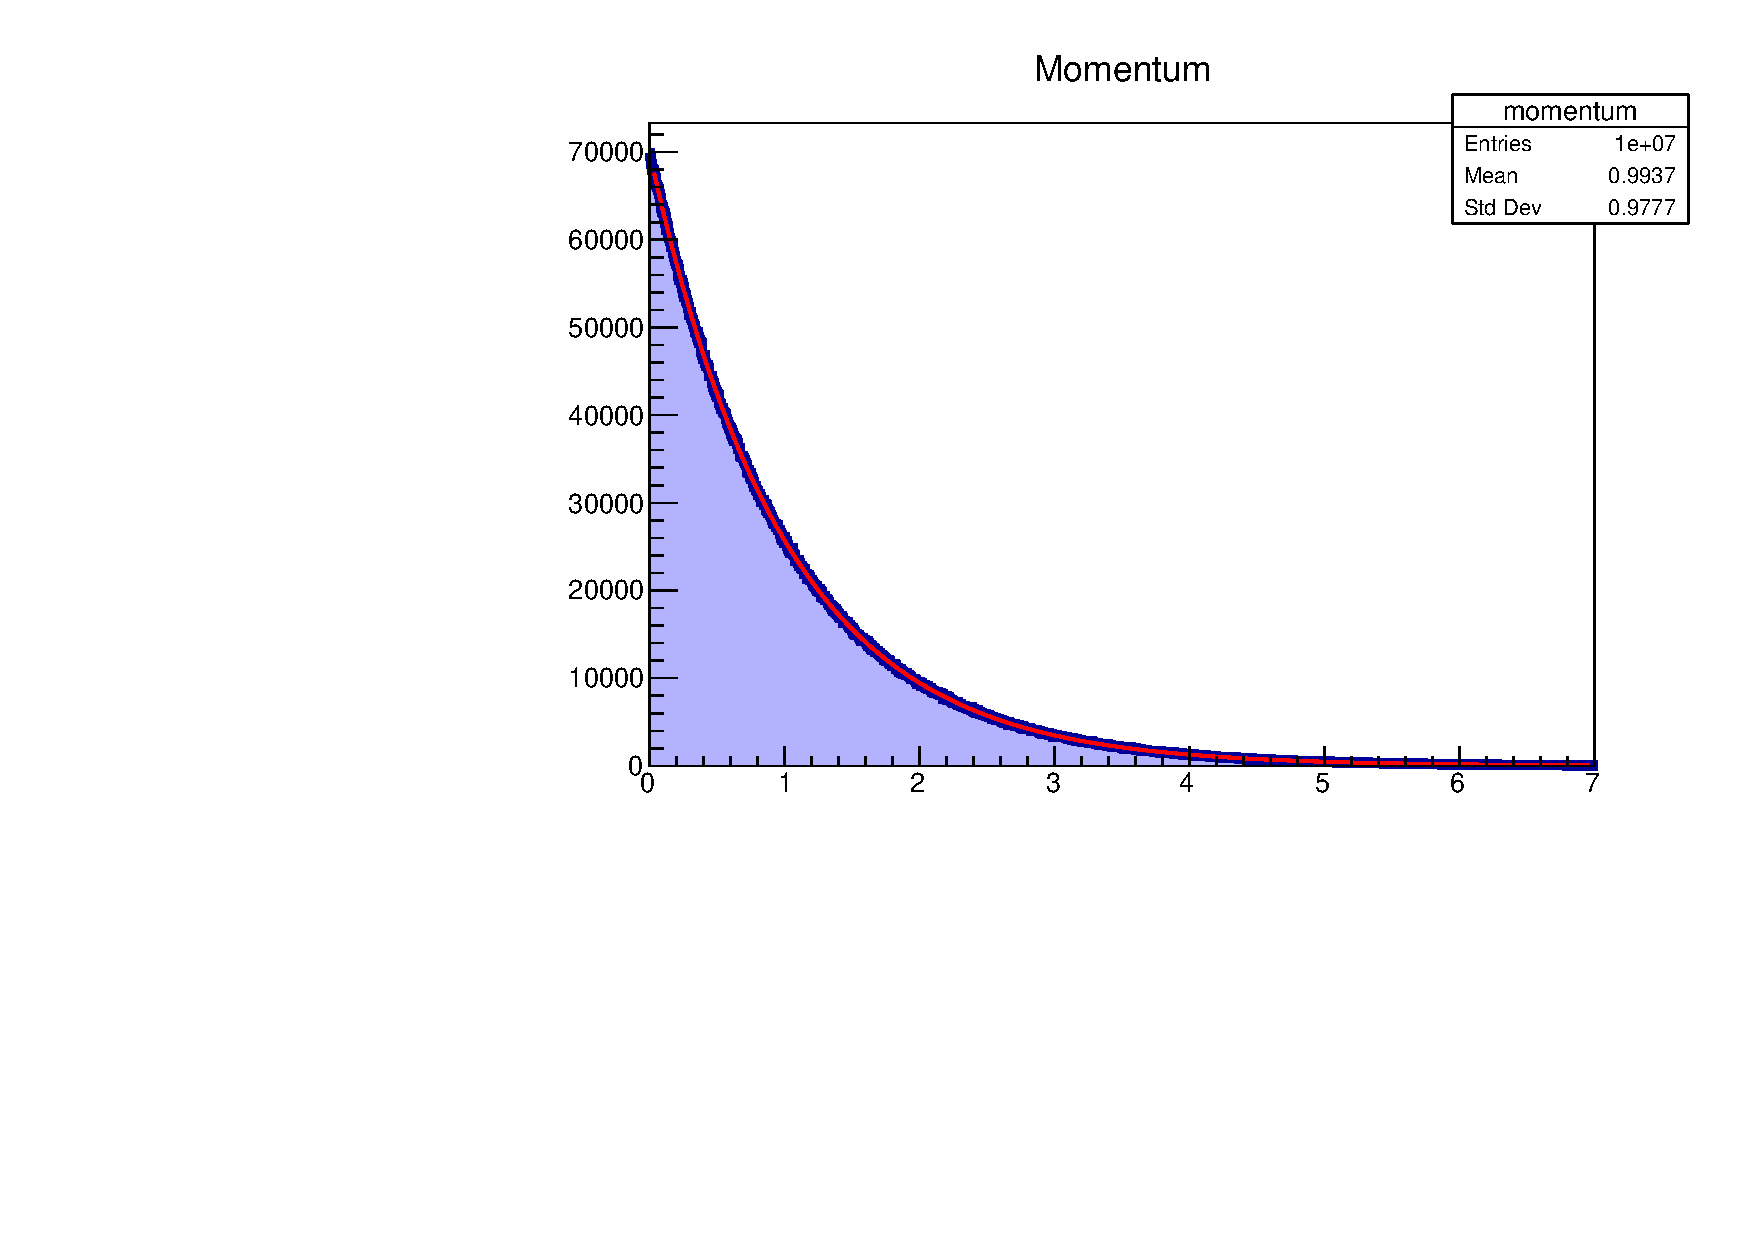
\includegraphics[width=9cm]{c1.pdf}
      \caption{\label{f1} \textit{The image shows the fit between the exponential distribution compared with the momentum histogram with occurrences randomly generated. The Chi-square divided by the number of degrees of freedom is very close to one, meaning that the histogram very well approximates an exponential distribution with a mean of 1.}}
    \end{figure}
    \begin{figure}
      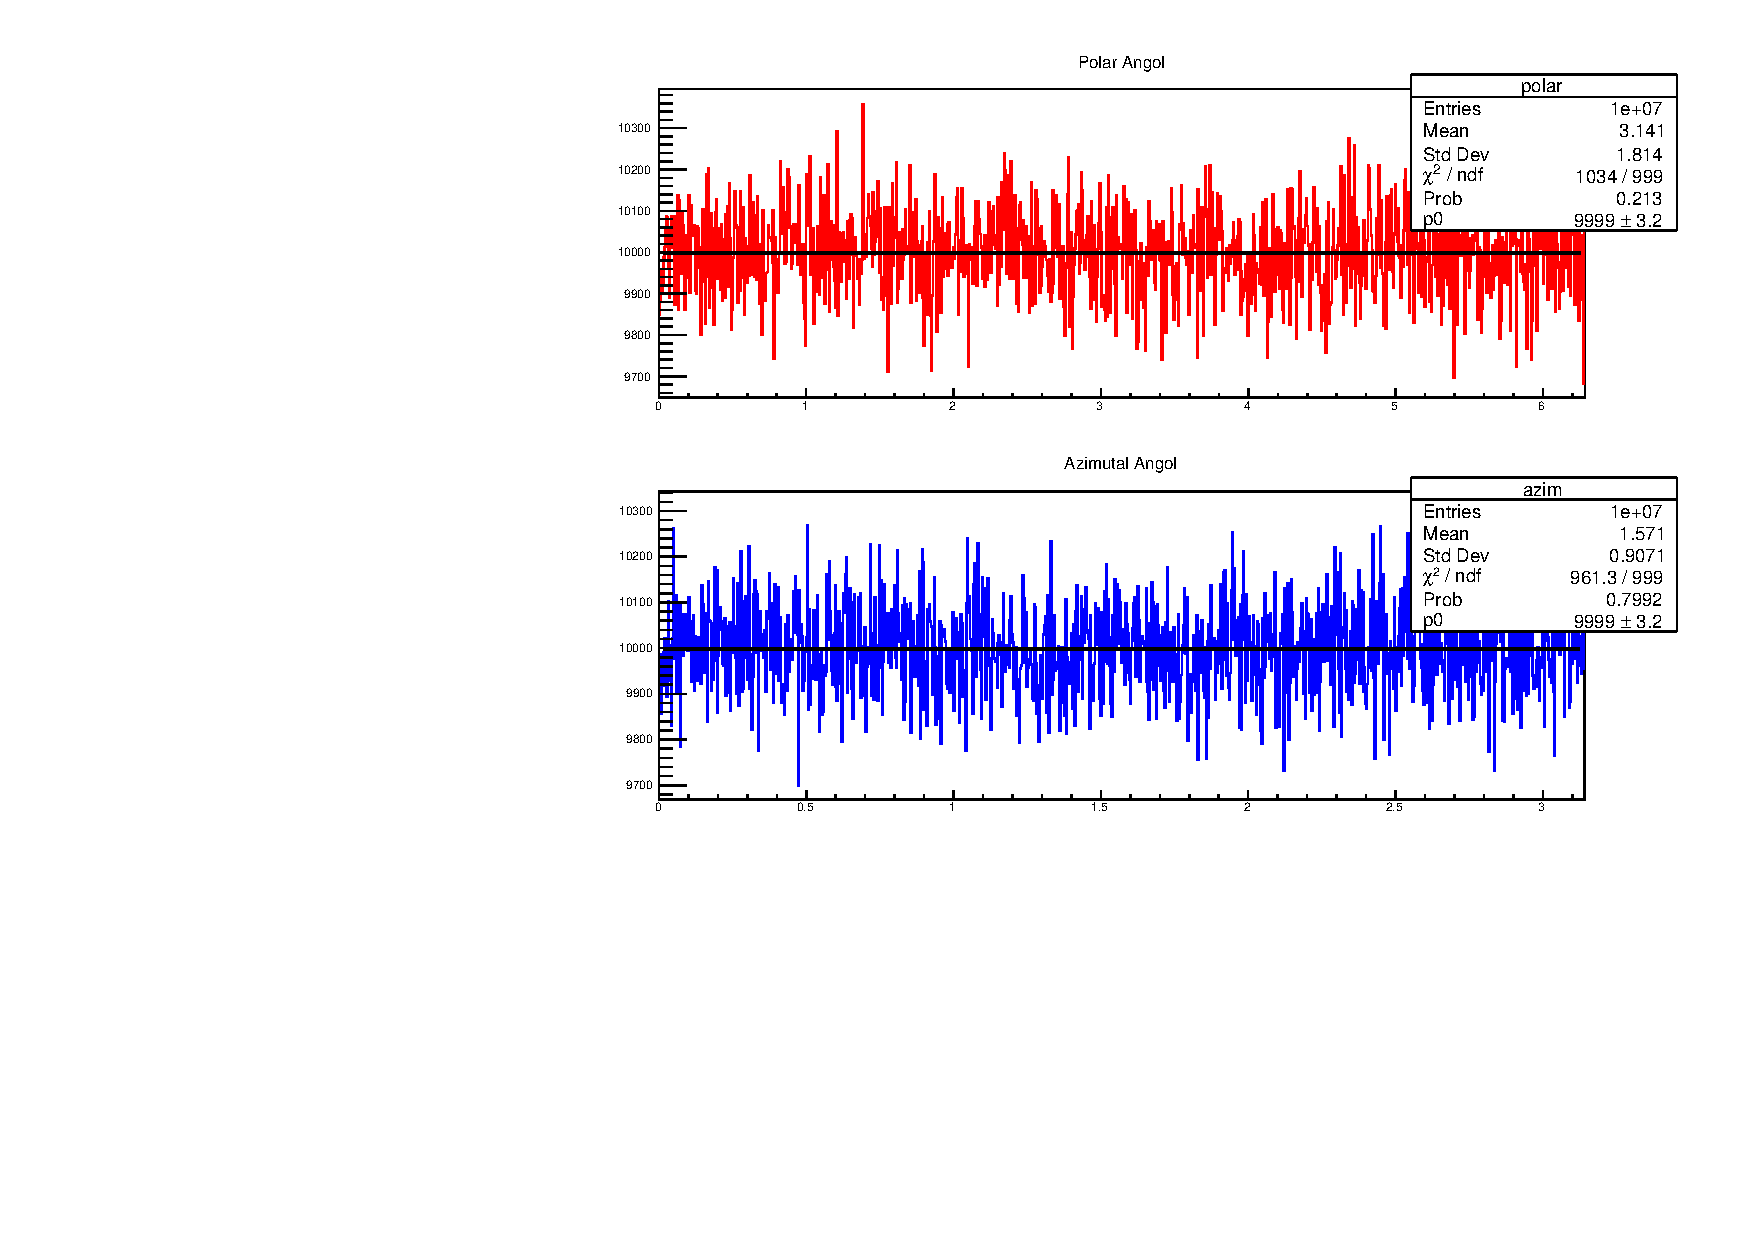
\includegraphics[width=9cm]{c2.pdf}
      \caption{\label{f1} \textit{The image shows the fit between the uniform distribution compared with the histogram of the angles randomly generated. The Chi-square divided by the number of degrees of freedom is very close to one, meanning that the histograms very well approximate an uniform distribution.}}
    \end{figure}
    \\
    \section* {Word Citacion}
    \begin{enumerate}
      \item{Alice Experiment. CERN. \url{https://home.cern/science/experiments/alice} . November $29^{th}$, 2021.}
    \end{enumerate}

\end{document}
